%%
%% This is file `mcmthesis-demo.tex',
%% generated with the docstrip utility.
%%
%% The original source files were:
%%
%% mcmthesis.dtx  (with options: `demo')
%% !Mode:: "TeX:UTF-8"
%% -----------------------------------
%% This is a generated file.
%% 
%% Copyright (C) 2010 -- 2015 by latexstudio
%%       2014 -- 2019 by Liam Huang
%%       2019 -- present by latexstudio.net
%% 
%% License: The LaTeX Project Public License 1.3c
%% 
%% The Current Maintainer of this work is latexstudio.net.
%% 

\documentclass{mcmthesis}
 %\documentclass[CTeX = true]{mcmthesis}  % 当使用 CTeX 套装时请注释上一行使用该行的设置
\mcmsetup{tstyle=\color{red}\bfseries,%修改题号,队号的颜色和加粗显示,黑色可以修改为 black
        tcn = 2524908, problem = C, %修改队号,参赛题号
        sheet = true, titleinsheet = false, keywordsinsheet = true,%修改sheet显示信息
        titlepage = false, abstract = true}

  %四款字体可以选择
  %\usepackage{times}
  %\usepackage{newtxtext,newtxmath} %CTeX 无此字体,可用 txfonts 替代,请使用新版 TeXLive.
 \usepackage[utf8]{inputenc}
 \usepackage{palatino}
  %\usepackage{txfonts}
\usepackage{float}
\usepackage{graphicx}
\usepackage{tabularx}
\graphicspath{ {./figures/} }
\usepackage{indentfirst}  %首行缩进,注释掉,首行就不再缩进。
\usepackage{lipsum}
\usepackage{tikz}
\usetikzlibrary{shapes.geometric, arrows}
\tikzstyle{startstop} = [rectangle, rounded corners, text centered, draw=black, fill=red!30]
\tikzstyle{process} = [rectangle, text centered, draw=black, fill=blue!30]
\tikzstyle{arrow} = [thick,->,>=stealth]
\title{MCM Problem C}
\author{\small \href{https://www.latexstudio.net/}
  {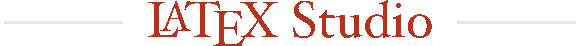
\includegraphics{mcmthesis-logo}}}
\date{\today}
\usepackage{hyperref}
\begin{document}
\begin{abstract}
\par %Use this template to begin typing the first page (summary page) of your electronic report. This
%template uses a 12-point Times New Roman font. Submit your paper as an Adobe PDF
%electronic file (e.g. 1111111.pdf), typed in English, with a readable font of at least 12-point type. 

%Do not include the name of your school, advisor, or team members on this or any page. 

%Be sure to change the control number and problem choice above. 

%You may delete these instructions as you begin to type your report here.  

%\textbf{Follow us @COMAPMath on Twitter or COMAPCHINAOFFICIAL on Weibo for the
%most up to date contest information.}

\begin{keywords}
Multiple Linear Regression; Neural Network; Entropy-weighted Method
\end{keywords}
\end{abstract}
\maketitle
%% Generate the Table of Contents, if it's needed.
\tableofcontents
\newpage
%%
%% Generate the Memorandum, if it's needed.
%% \memoto{\LaTeX{}studio}
%% \memofrom{Liam Huang}
%% \memosubject{Happy \TeX{}ing!}
%% \memodate{\today}
%% \memologo{\LARGE I'm pretending to be a LOGO!}
%% \begin{memo}[Memorandum]
%%   \lipsum[1-3]
%% \end{memo}
%%
\section{Introduction}

\subsection{Background}

The Olympic Games have long served as a global stage where athletes from diverse backgrounds come together to compete at the highest level. Scheduled to take place in Los Angeles, California, the 2028 Summer Olympics mark the city’s third time hosting this prestigious event, following its successful iterations in 1932 and 1984.

As the Games approach, attention is increasingly focused on the potential medal outcomes, which reflect not only the athletes’ dedication but also the geopolitical, cultural, and economic forces shaping global sports. Nations are investing heavily in sports programs, science-backed training methods, and athlete development, with the aim of achieving their position on the medal table. At the same time, emerging powers in international sports are challenging the dominance of traditional medal-winning nations, hinting at a potential reshaping of the competitive landscape in 2028.

This paper explores these dynamics within the unique context of the Los Angeles Games, including its innovative event lineup, the past performances of each country and the composition of each national team.

\subsection{Framework of Analysis}
In this paper, we established multiple models to predict the medals earned of each country in the 2028 Olympic Games held in Los Angeles. The first model we take is the artificial neural network (ANN). The neural network program is constructed using Python and trained with the databases provided by the organizer of this competition. The databases we used included data about the names of athletes and the countries they represent, the hosting country, the medals awarded, and the hosting year from 1896 to 2024 of each country. The other model we take is multiple linear regression (MLR). In this model, we find the linear relationships between the variables in the database and the medals earned of each country. To find the synthetic results from these two outcomes of different methods, we take the entropy-weight method (EWM) to calculate the weight between the data from each method. Eventually, we will take the weighted average value to obtain the final result.  

\subsection{Comments on Data Provided}
There have been many inconsistencies we observed in the provided data, many of which were not addressed in the problem statement. Nonetheless, we have found ways to circumvent these errors to create working models regardless. First, we must address the issue of the 1906 Summer Olympics. While running tests on the multidimensional regression model we found an error in which the model handled one specific date, namely the 1906 Olympics. After closer reading, it came to out attention that the 1906 Olympics did not follow the standard 4 year gap between events. This was cumbersome because this information was only stored in the athletes data file, and not mentioned in neither the medal count file nor the host file. This deleted crucial information on which the regression model bases its predictions on. We have elected not to include those Olympics in the regression model, due to the stipulation not to use any external data (i.e. data from sources others than the ones provided). It had been included, however, in the neural network model, as there need not be for extremely precise definitions compared to the regression model; however, this might be contributing to some amount of error (formally called \textit{loss} in machine learning environments).
We have also found errors in the files themselves. There are certain characters at the end of some team names that inhibit complete data analysis on the unmodified provided files. These include, but are not limited to, the characters " " being concatenated to the end of country names in the \texttt{medal\_counts.csv} file for the 1932 and 1960 Olympics, the existence of "subteams" like Japan-1 or United States-13, or the aforementioned lack of host data for the special 1906 Summer Olympics. Although it is difficult to predict what influence these errors had on the neural network model, we found ways to circumvent these issues when working with the regression model. 

\section{Analysis of the Problem}

\subsection{The Artificial Neural Network}
The artificial neural network was coded in Python 3.12.0, with the help of standard machine learning (ML) and data analysis libraries: \href{https://pandas.pydata.org/}{\texttt{Pandas}}, \href{https://numpy.org/}{\texttt{NumPy}}, \href{https://scikit-learn.org/stable/}{\texttt{scikit-learn}} and \href{https://www.tensorflow.org/}{\texttt{TensorFlow}}. The raw code may be found in Appendix A after following the github link. The Artificial Neural Network (henceforth abbreviated as ANN) was trained on three of the four provided files: \texttt{summerOly\_atheletes.csv}, \texttt{summerOly\_hosts.csv}, \\ \texttt{summerOly\_medal\_counts.csv}. The ANN was designed with three layers, the input layer (with 32 neurons), the middle layer (with 16 neurons) and the output layer (with 1 neuron). After each training iteration, the ANN prunes (omits) random neurons and connections (20\% for this ANN) to prevent overfitting and force the ANN to learn the patterns visible in the training data. This is done to prevent the ANN from depending on any specific neuron, which is common in smaller ANN's (like the one created for this paper) or with a relatively small amount of training data (also the case in this problem). An example of a pruned neural network is shown in Figure~\ref{figure: NN}. The data followed the standard 90/10 split, whereby 90\% of the data was used to train the model, and 10\% to test the models accuracy. Rectified Linear Unit (ReLU) was chosen as the activation function for the first 2 ANN layers, due to the many benefits it provides over other functions like Sigmoid, which tend to slow the model down during backpropagation, since it confines all inputs into the range $[0, 1]$. For very large or small input values, the gradient is disproportionally closer to 0, which significantly slows down the updating of weights between neurons. Although many slightly different variations of the ReLU function exist, the ANN used the function defined as $x\mapsto \max(0, x)$.

\begin{figure} [H]
    \centering
    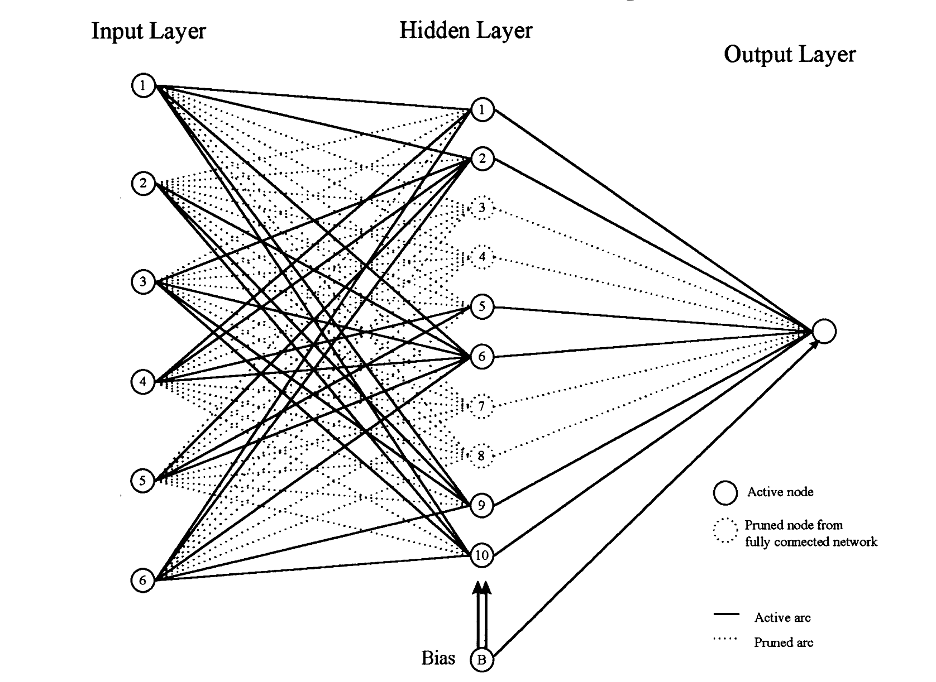
\includegraphics[width=0.95\textwidth]{prunes-nn-vis}
    \caption{Example of pruned neural network}
    \label{exampleID}
    \label{figure: NN}
\end{figure}

The final layer was standardized using the Softmax function, again as is custom in multilayer classification neural networks. Softmax standardizes the outputs to be a valid probability distribution, defined as:
\begin{equation}\label{eq:softmax}
    \text{Softmax}(z_i) = \frac{e^{z_i}}{\sum_{j=1}^{n} e^{z_j}}
\end{equation}
The ANN also used three additional functions to calculate its effectiveness. The optimizer Adam (Adaptive Moment Estimation) function was used to minimize the loss function dynamically, by changing the weights and biases of neurons and connections. It ensures the neural network converges to a good solution efficiently. It is defined mathematically below:
\begin{align}\label{eq:adam func}
    \begin{split}
    &\omega_{t+1}=\omega_t-\alpha m_t\\
    &m_t = \beta m_{t+1} + (1-\beta) \left[\frac{\partial L}{\partial \omega_t} \right]
    \end{split}
\end{align}

\begin{table}[H]
\caption{Variable Definitions for Equation~(\ref{eq:adam func})}
\centering
\begin{tabularx}{\textwidth} {
  >{\raggedright\arraybackslash}X 
  >{\raggedright\arraybackslash}X  }
 \hline
 \textbf{Variable} & \textbf{Definition} \\
 \hline\hline
  $t_0$ & Initial time, $t_0 = 0$ \\
 $m_t$ & Aggregate of gradients at $t$ ($m_{t_0}=0$) \\
 $m_{t-1}$ & Aggregate of gradients at $t_{previous}$ \\
 $\omega_{t}$ & Weights at $t$ \\ 
 $\omega_{t+1}$ & Weights at $t\equiv t+1$ \\ 
 $\alpha_t$ & Learning rate at $t$ \\ 
 $\partial L$ & Derivative of the loss function \\ 
 $\partial \omega_t$ & Derivative of weights at $t$ \\
 $\beta$ & Moving average parameter, const. \\
 \hline
\end{tabularx}
\end{table}

The loss function was chosen to be \textit{Binary Cross Entropy} (also known as \textit{log loss}). The neural network was punished when loss was high, which leads to the ANN learning the data. The Binary Cross Entropy function is defined as:
\begin{equation}\label{eq:binary crossentropy}
    \text{BCE} = -\frac{1}{N}\sum_{i=0}^{N}\left [y_i \log(p_i) +(1-y_i)\log(1-p_i)\right]
\end{equation}

\begin{table}[H]
\caption{Variable definition for eqn~(\ref{eq:binary crossentropy})}
\centering
\vspace{5pt}
\begin{tabularx}{\textwidth} {
  >{\raggedright\arraybackslash}X 
  >{\raggedright\arraybackslash}X  }
 \hline
 \textbf{Variable} & \textbf{Definition} \\
 \hline\hline
  $N$ & Number of instances \\
  $y_i$ & True label for instance $i$ \\
 $p_i$ & Model predicted probability of instance $i$ \\ \hline
 \end{tabularx}
\end{table}

\subsubsection{Results}

Full results of ANN predictions may be found in Section~\ref{RestultsIntegration}. This section will be dedicated to providing the results for the ANN itself. The ANN used $n=50$ epochs for training, to ensure maximum accuracy of the model and minimize the risk of potential overfitting. The final values for key metrics are shown in the table below.

\begin{table}[H]
\caption{Key ANN metrics}
\centering
\vspace{5pt}
\begin{tabularx}{\textwidth} {
  >{\raggedright\arraybackslash}X 
  >{\raggedright\arraybackslash}X  }
\hline
 \textbf{Metric} & \textbf{Value} \\   
 \hline\hline
  Training Accuracy & $0.9976$\\ 
  Training Loss & $0.0173$\\
 Validation Accuracy & $0.9250$\\
 Validation Loss & $0.2187$\\ \hline
\end{tabularx}
\end{table}

Although it is not possible to fully understand how the neural network learned the data, the four above metrics give insight into its workings on both training and validation (testing) data. Looking at the training metrics first, it becomes clear the model handles seen data exceptionally well, with an extremely high training accuracy and very low training loss. Usually, this means the neural network is extremely well trained. In this case, however, it may point towards overfitting, since the winners of events are (somewhat) random. Having a $0.9976$ and $0.0173$ training accuracy and loss on a slightly random data set is a first indication of overfitting in the model. However, the ANN still fairs well with data it has not yet seen, as evidenced by the relatively high validation accuracy. The increase in loss value from training to validation does support the overfitting hypothesis, however it is well within accepted ranges for well trained neural networks, meaning the predictions of the ANN may be accepted as valid.

\subsection{Multiple Linear Regression}

\subsubsection{Data Processing}

\section{Results Integration}\label{RestultsIntegration}
\subsection{Determination evaluation indicators}
The final predictions obtained by the two methods above are shown in the table below:
\begin{table}[H]
\centering 
\label{A}
 \caption{Medals Earned of Each Country in 2028 Olympic Game}
\vspace{5pt}
\begin{tabular}{lcc}
\hline
\textbf{Name of Country} & \textbf{Artificial Neural Network} & \textbf{Multiple Linear Regression} \\
\hline\hline
United States & 144 & A\\
Great Britain & 60 & A\\
France & 42 & A\\
Italy & 28 & A\\
Germany & 23 & A\\ 
$\vdots$ & $\vdots$ & $\vdots$\\ 
Democratic Republic of the Congo & 0 & A\\
Wales & 0 & A\\
South Sudan & 0 & A\\
North Macedonia & 0 & A\\ 
\hline
\end{tabular}
\end{table}
\begin{figure}[h]
  \centering
  \includegraphics[example-image-a]{1} % 直接写图片名字,不需要后缀
  \caption{Distributions of medals earned of this two method }
  \label{exampleId}
\end{figure}
However, due to the differences of these two algorithm, there are many differences exist between the values obtained by different method. 

The prediction of the neural network was standardized relative to the number of disciplines projected to be in the 2028 Olympics. Clearly, if more events are in a given Olympic, the higher the total number of medals will be, and therefore the total number of medals won by each team will be greater. Since the events and teams for the 2028 Olympics have not yet been published, we were forced to make assumptions regarding these metrics. For the medal predictions, the values were adjusted based on the number of events we assume will happen in 2028, which we took to be the exact same as in 2024. The model does account, however, for a differing number of disciplines, and can be parsed into the function to change to predictions.

To solve the problem of differences in the data obtained from different methods, we need to use particular methods to combine these outcomes to get the results. To do this, we adapt the entropy-weighted method to calculate the synthetic result.

\subsection{Entropy Weight Method Model}
The entropy-weighted model is an evaluation model that determines the weights of various indicators based on the differences in the information contained in each indicator and combines the rankings derived from the proximity to the ideal solution. The specific operational flow chart is as follows:
\begin{figure}[H]
\centering
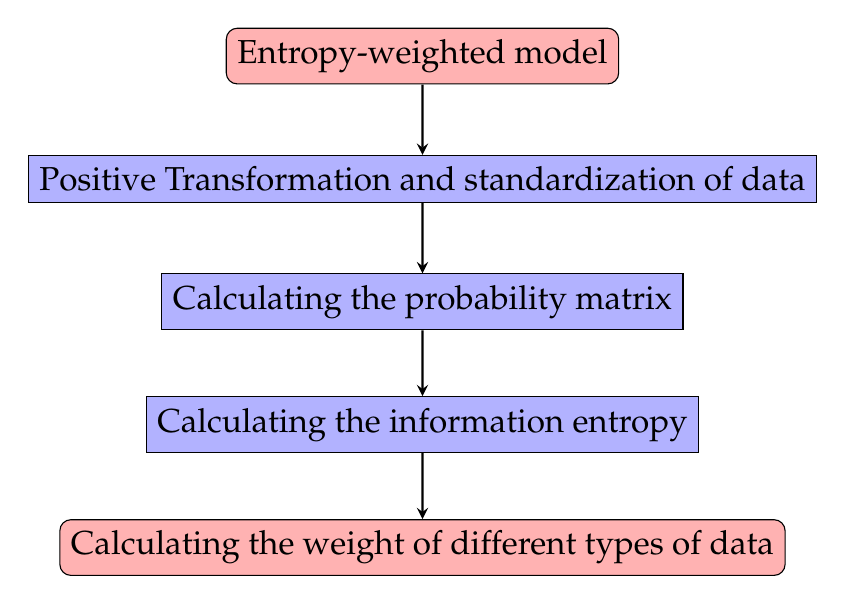
\begin{tikzpicture}[node distance=1.3cm, scale=1.2, transform shape] % 缩放到合适大小
% 定义节点
\node (start) [startstop] {Entropy-weighted model};
\node (step1) [process, below of=start] {Positive Transformation and standardization of data};
\node (step2) [process, below of=step1] {Calculating the probability matrix};
\node (step3) [process, below of=step2] {Calculating the information entropy };
\node (stop) [startstop, below of=step3] {Calculating the weight of different types of data};

% 添加箭头
\draw [arrow] (start) -- (step1);
\draw [arrow] (step1) -- (step2);
\draw [arrow] (step2) -- (step3);
\draw [arrow] (step3) -- (stop);
\end{tikzpicture}
\caption{Flowchart of The Process of EWM}
\label{fig:flowchart}
\end{figure}
In most previous competitions, most countries didn`t win any medals, and only very few countries gained the most medals, which looks like a Gamma distribution. Thus, the criteria to determine which result is more likely to be correct is to see which results match the Gamma distribution.\\
\begin{equation}\label{eq:1}
f(x;k,\theta) =\frac{1}{\Gamma(k) \theta^k}x^{k-1}e^{-\frac{x}{\theta}}.
\end{equation}
In this case, we are going to do the positive transformation by using the formula below:
\begin{equation}\label{K}
x_i = \frac{f(x_i) - \min(f(x))}{\max(f(x)) - \min(f(x))}
\end{equation}
The $x_i$ in(\ref{K}) is the number of medals a particular country gains under a specific method. The data after the positive transformation is in the table below:
\begin{table}[H]
\centering 
\label{A}
\caption{Data about medals earned after positive transformation}
\vspace{5pt}
\begin{tabular}{lcc}
\hline
\textbf{Name of the Country} & \textbf{Artificial Neural Network} & \textbf{Multiple Linear Regression} \\
\hline\hline
\end{tabular}
\end{table}
After the positive transformation, we need to normalize the data by using the formula below:\\
\begin{equation}\label{V}
\hat{x}_i=\frac{x_i}{\sqrt{x_{1}^{2}+x_{2}^{2}+\cdots+x_{n}^{2}}}
\end{equation}
In the formula~\eqref{V}, $n$ is the number of the country. Since we obtain the medals earned by using two different method, we can use a two-dimension matrix to contain these value:\\
\begin{equation}\label{eq:3}
\tilde{x}=
\begin{bmatrix}
	x_{11}&		x_{12}\\
	x_{21}&		x_{22}\\
	\vdots&		\vdots\\
	x_{(n-1)1}&		x_{(n-1)2}\\
	x_{n1}&		x_{n2}\\
\end{bmatrix}
\end{equation}
The first column represents the medals earned as a prediction from the artificial neural network, and the second column represents the medals earned from the prediction of multiple linear regression.
Now, our goal changes to find the matrix:
\begin{equation}\label{eq:3}
\tilde{z}=
\begin{bmatrix}
	z_{11}&		z_{12}\\
	z_{21}&		z_{22}\\
	\vdots&		\vdots\\
	z_{\left( n-1 \right) 1}&		z_{\left( n-1 \right) 2}\\
	z_{n1}&		z_{n2}\\
\end{bmatrix}
\end{equation}
where
\begin{equation}\label{eq:1}
z_{ij}=\frac{x_{ij}}{\sqrt{x_{1j}^{2}+x_{2j}^{2}+\cdots+x_{nj}^{2}}}
\end{equation}
After gaining the normalized data of the medals earned, we calculating the Weight matrix:
\begin{equation}\label{eq:3}
\tilde{p}= 
\begin{bmatrix}
	p_{11}&		p_{12}\\
	p_{21}&		p_{22}\\
	\vdots&		\vdots\\
	p_{(n-1) 1}&		p_{\left( n-1 \right) 2}\\
	p_{n1}&		p_{n2}\\
\end{bmatrix}
\end{equation}
where
\begin{equation}\label{eq:1}
\tilde{p}_{ij}=\frac{z_{ij}}{\sum_{i=1}^n z_{ij}}
\end{equation}
And then, we calculate the information entropy, $e_j$ of each method (ANN and MLR):
\begin{equation}\label{eq:1}
e_j=-\frac{1}{\ln n}\sum_{i=1}^n p_{ij}\ln (p_{ij}) \quad \left( j=1,2 \right)  
\end{equation}
Then, we calculate the information utility value of each type of method (ANN and MLR):
\begin{equation}\label{eq:1}
d_j=1-e_j.  
\end{equation}
Finally, we get the weight of each method by normalizing the utility values:
\begin{equation}\label{eq:1}
w_j=\frac{d_j}{d_1+d_2} \quad (j=1,2)
\end{equation}
The entropy-weighted method was coded in Python 3.12.6 with data analysis libraries NumPy, SciPy, and Pandas. The weights of each method are shown in the table below.
\begin{table}[H]
\centering 
\label{B}
\caption{Weight of Each Method}
\vspace{5pt}
\begin{tabularx}{\textwidth} {
  >{\raggedright\arraybackslash}X 
  >{\raggedright\arraybackslash}X  }
\hline
\textbf{Artificial Neural Network} & \textbf{Multiple Linear Regression} \\
\hline\hline
\end{tabularx}
\end{table}
Based on the composite weights, we calculate the weighted average of the medaas earned obtained by different methods for the same country:
\begin{equation}\label{eq:1}
\text{Medals earned} = w_\text{ANN}R_\text{ANN} + w_\text{MLR}R_\text{MLR}.
\end{equation}
 $R_{}$ is the total medals earned by a certain country calculated by the artificial neural network, and $R_(MLR)$ is the total medals earned by the same country calculated by the multiple linear regression.\\
We use this to derive the final medals earned for each country as show in the table below:
\begin{table}[H]
\centering 
\label{c}
\caption{Medals Earned from Each Country}
\vspace{5pt}
\begin{tabularx}{\textwidth} {
  >{\raggedright\arraybackslash}X 
  >{\raggedright\arraybackslash}X  }
 \hline
\textbf{Name of the country} & \textbf{Medals earned} \\
\hline\hline
\end{tabularx}
\end{table}






\section{Validating the Model}


\section{Conclusions}




\section{Evaluation of the Model}
Certain features of the models used in this paper work better for different questions one may have regarding the 2028 Olympics medal distribution. In truth, a combination of the ANN and MLR is useful for a more rounded overall model. While certain predictions are consistent across both models, there are crucial differences which make one better than the other in certain aspects. For example, the ANN model predicts that no new countries will win a medal in the 2028 Olympics, and it is quite easy to understand why. The model has learned that over the span of 128 years and 32 Summer Olympic Events, a particular country has not won once. On the basis of that knowledge, there is no reason why it should suggest that suddenly a country may win a medal. In this case, the linear regression model reigns supreme, as it operates on an entirely different basis, as does not fall short to the situation described above. Conversely, finding relationships of specific variables, rather than entire datasets, the MLR model is able to more accurately predict whether a country will win its first medal based on its attributes. Another consequence of the ANN learning entire data sets is a possible erroneous prediction of certain team medals. For instance, China has taken part in merely 11 Olympics, as opposed to the United States which took part in almost 30. This results in the ANN assigning China 0 medals for all Olympics it had not participated in, reinforcing a notion that China's recent successes a merely a fluke, not replicable in future events. Again, in such situations the MLR has an advantage over the ANN. The ANN model works better for conclusions requiring a view on the whole set of data, such as the influence of \textit{Host Advantage}. The MLR tries to account for this metric, but finds very little correlation, since it bases its predictions on only 1 Summer Olympic prior. This may explain the reason for a bigger discrepancy for the number of medals won by the United States than for any other country - perhaps the ANN found support for Host Advantage playing a role, and predicts the United States, as a host of the 2028 Los Angeles Olympics, will earn more medals. Many such differences exist between the two models, which is why we elected to construct both in harmony with each other. Their collective predictions should be a much more trust-worthy metric, as compared to both models in solitude.
\section{Strengths and weaknesses}


\subsection{Strengths}
\begin{itemize}
\item{}
\end{itemize}

\subsection{Weaknesses}
\begin{itemize}
\item {Gamma distribution might not be able to exactly describe the distribution of the medals earned of each country}
\item {The ANN model takes into account all historical data, and sometimes predicts countries like the Soviet Union, Yugoslavia or Czechoslovakia as a possible winner. While the model ranks these countries very low, it ranks them nonetheless, meaning it may in theory predict that a non-existent country will win a medal, which is impossible.}
\item \\

\item \\

\end{itemize}

\begin{thebibliography}{99}

\end{thebibliography}

\begin{appendices}

\section{First appendix}

\section{Second appendix}

\end{appendices}

\AImatter

\begin{ReportAiUse}{9}

\end{ReportAiUse}

\end{document}
%% 
%% This work consists of these files mcmthesis.dtx,
%%                                   figures/ and
%%                                   code/,
%% and the derived files             mcmthesis.cls,
%%                                   mcmthesis-demo.tex,
%%                                   README,
%%                                   LICENSE,
%%                                   mcmthesis.pdf and
%%                                   mcmthesis-demo.pdf.
%%
%% End of file `mcmthesis-demo.tex'.
